% 第 2 章 物联网数据采集场景
\chapter{物联网数据采集场景}

工业与园区场景中，数据采集是数字化底座的第一公里。本章基于 EdgeFlow v0.1.0 已实现能力，阐述以边缘就近采集为核心的方案设计、特性引用、部署方式与客户价值。

\section{业务痛点}

以下痛点基于工业/园区场景的通用行业实践（不涉及具体客户）：

\begin{itemize}
  \item \textbf{设备协议异构，接入成本高}：工厂与园区内传感器、PLC、仪表、控制器等设备品牌繁杂，通信协议各异（Modbus、私有协议等）。每接入一类设备往往需要一套定制集成，重复建设、周期长，形成数据孤岛。
  \item \textbf{采集链路脆弱，单点依赖公网}：传统架构下设备数据经边缘逐级上送云端，任一环节（公网波动、云端故障）都会导致采集中断，现场业务“断网即停”。
  \item \textbf{全量上云，成本与时效失衡}：原始数据全量上云带来带宽与存储成本，而大量状态类数据只需周期性快照；高频采集与有限带宽之间存在矛盾。
  \item \textbf{运维黑盒，问题定位困难}：设备状态、指令执行结果、采集错误缺乏统一记录，现场排查依赖人工，故障不可追溯。
\end{itemize}

\section{方案设计}

EdgeFlow 采用“\textbf{边缘就近采集、数据面与管理面分离、影子汇聚、周期上报}”的架构：

\begin{itemize}
  \item \textbf{边缘就近采集（本地优先）}：edgecore 部署于边缘节点，通过 Mapper 适配层对接现场设备。Modbus TCP 设备经本地网络直连（F26），采集链路不依赖公网，断云不影响采集；MQTT 数据面独立于云边管理面。
  \item \textbf{Mapper 适配层}：以 DeviceMapper 接口 + MapperRegistry 路由/生命周期管理（F24）实现协议适配；内置温湿度模拟 Mapper（F25）与 Modbus TCP Mapper（F26），新增协议以 Mapper 方式扩展。
  \item \textbf{MQTT 数据面}：EventBus 以 MQTT 承载遥测/指令主题，QoS1 至少一次投递（F28），消费方需自行幂等；broker 不可用时自动降级纯本地模式、进程不退出（F29）。
  \item \textbf{影子汇聚}：DeviceTwin 影子自动创建，合并 desired/reported（F21），边缘影子始终为最新值；设备属性按周期上报云端（F22），云端视图由上报构建（设备状态为云端内存态）。
  \item \textbf{指令闭环}：device-command 经可靠投递到达 Mapper 直接执行，并写回 Desired（F23），指令执行链路可追踪。
\end{itemize}

\section{产品特性引用}

\textbf{表 2-1：数据采集场景特性引用}

{\small\setlength{\tabcolsep}{3pt}
\begin{tabular}{@{}p{1.6cm}p{0.8cm}p{6.4cm}p{5.8cm}@{}}
\toprule
场景需求 & 特性 & 能力说明 & 部署要点\\
\midrule
协议异构设备统一接入 & F24 & DeviceMapper 接口 + MapperRegistry 负责 Mapper 的路由与生命周期 & 按协议实现 Mapper 并在 edgecore 启动时挂载\\
温湿度类设备接入与演示 & F25 & mock\_sensor 模拟温湿度，2s 波动；支持 targetTemp/reset 指令，收敛+随机扰动 & 联调/演示开箱即用，无需实体设备\\
Modbus 设备接入 & F26 & Modbus TCP Mapper：读写保持寄存器/线圈，写后回读验证，错误落 op-ledger & 显式 opt-in：须设置 \env{EDGEFLOW\_MODBUS\_ADDR} 才注册\\
遥测与指令数据面 & F28 & MQTT 遥测/指令主题，QoS1（至少一次、不保证去重，消费方需幂等）；paho 自动重连+订阅恢复 & 配置 MQTT broker；数据面独立于云边管理面\\
数据面容错 & F29 & broker 不可用自动降级纯本地模式，进程不退出 & 降级后恢复需重启 edgecore\\
设备影子 & F21 & desired/reported 合并、深拷贝、自动创建 & 无需预建，首次上报自动创建\\
属性周期上报 & F22 & 默认 30s 上报一轮，启动即报 & 可用 \env{EDGEFLOW\_EDGECORE\_DEVICE\_REPORT\_INTERVAL} 调整（1s--10min）\\
操作台账 & F27 & op-ledger 设备操作流水（SQLite 追加，30 天保留）：采集/下发方向、结果与错误 & 采集与指令操作自动落台账，Modbus 错误 result=error\\
指令可靠闭环 & F23 & \seqsplit{\texttt{POST /api/v1/nodes/\{nodeID\}/device-command}}：可靠投递（5s 超时、最多 3 次尝试、同 ID 重发、幂等去重）$\rightarrow$ Mapper 直接执行 $\rightarrow$ 写 Desired & 依赖云边通道可靠投递（F01/F05）承载\\
设备视图查询 & F30 & GET /api/v1/devices、GET /api/v1/nodes/\{nodeID\}/devices & 用于验证设备接入与属性可见性\\
\bottomrule
\end{tabular}}

\begin{quote}
注：本表收录 F21--F30 中经事实基线核验的条目；F01/F05 为指令链路所依赖的云边通道能力。
\end{quote}

\textbf{边界说明（如实口径）}：

\begin{itemize}
  \item 设备级离线检测\textbf{规划中}：当前无设备离线判定机制；Mapper 采集失败仅记 Warn，本轮按旧值上报；Modbus 读写错误落 op-ledger（result=error），需结合台账/日志人工定位。
  \item 云端设备状态为内存态，重启后依赖边缘周期上报重建（详见第 3 章）。
\end{itemize}

\section{部署方式}

\begin{figure}[htbp]
  \centering
  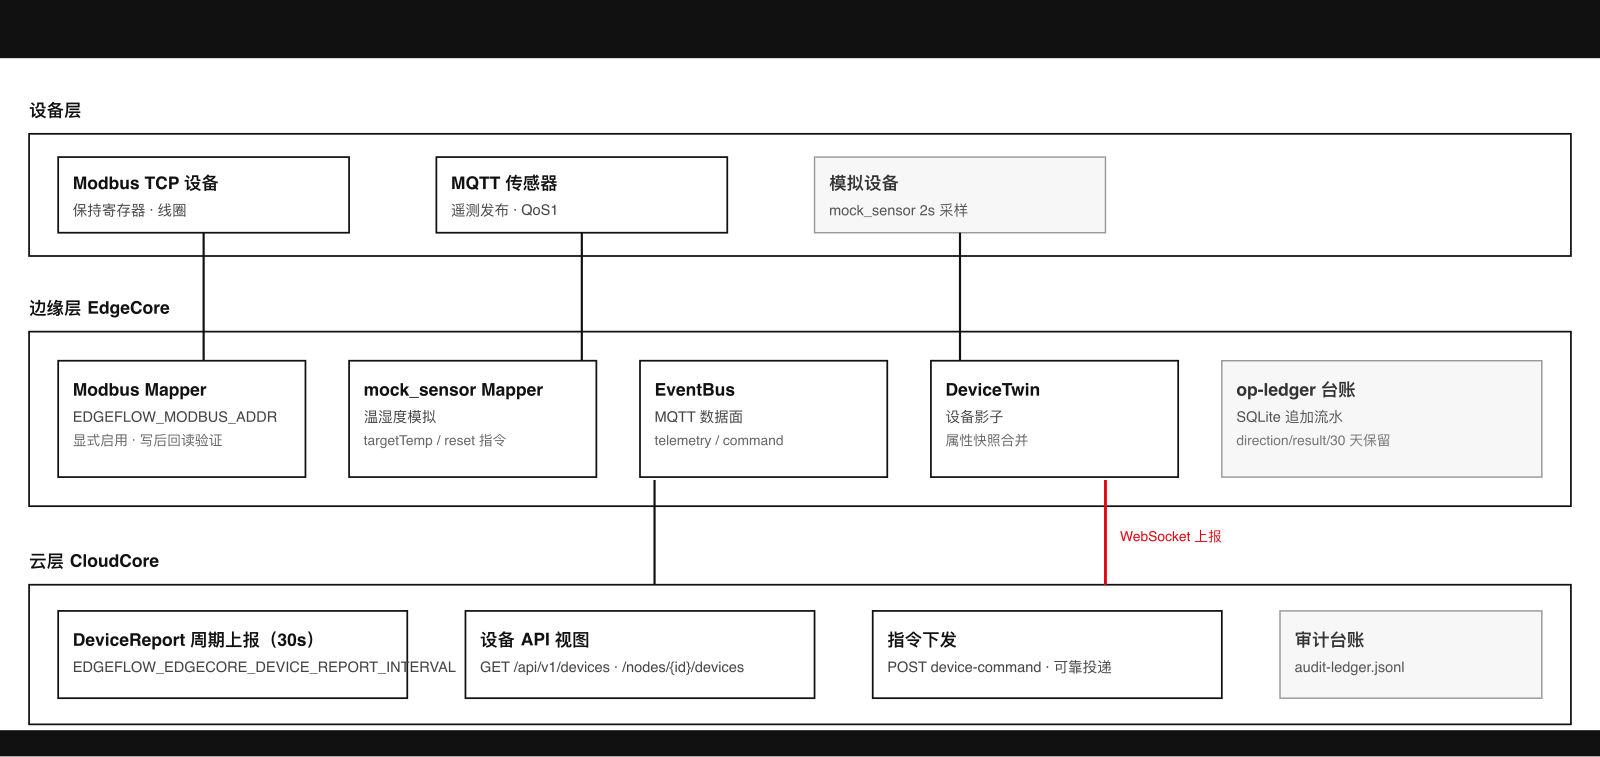
\includegraphics[width=0.94\textwidth]{../diagrams/scenario-collect.png}
  \caption{物联网数据采集场景部署拓扑}
  \label{fig:collect}
\end{figure}

以“边缘节点 + Modbus 设备（或 mock\_sensor 模拟）”为例：

\begin{enumerate}
  \item \textbf{部署 edgecore}：在边缘节点安装并启动 edgecore，确保与现场设备处于同一本地网络。
  \item \textbf{启用 Mapper}：
  \begin{itemize}
    \item 联调环境可直接使用 mock\_sensor（F25），开箱即得温湿度数据与 targetTemp/reset 指令；
    \item 接入真实 Modbus 设备时，设置环境变量 \env{EDGEFLOW\_MODBUS\_ADDR} 显式启用 Modbus TCP Mapper（F26，不设置则不注册）。
  \end{itemize}
  \item \textbf{配置 MQTT 数据面}：配置 MQTT broker（遥测/指令主题，QoS1，F28）。broker 不可用时 edgecore 自动降级纯本地模式继续运行（F29）；恢复后需重启 edgecore。
  \item \textbf{配置上报周期}（可选）：设置 \env{EDGEFLOW\_EDGECORE\_DEVICE\_REPORT\_INTERVAL}（1s--10min，默认 30s；启动即报一轮，F22），或写入 edgecore 配置文件 \seqsplit{\texttt{config/edgecore.json}}（cloudAddr/podReportInterval/deviceReportInterval/reconcileInterval 4 字段，\texttt{--config} 可指定路径；优先级：环境变量 > 配置文件 > 默认值，敏感配置如 Token 仅走环境变量）。上报周期变更支持热重载（SIGHUP 立即重载或 $\leq$60s 自动检测生效，无需重启；重载失败保持旧配置继续运行，fail-safe），详见 3.4。
  \item \textbf{验证}：
  \begin{itemize}
    \item \texttt{GET /api/v1/devices} 查看设备与属性（影子数据，F30）；
    \item \texttt{GET /api/v1/nodes/\{nodeID\}/devices} 按节点查看设备（F30）；
    \item \texttt{POST /api/v1/nodes/\{nodeID\}/device-command} 下发指令（如 mock\_sensor 的 targetTemp），验证可靠投递（5s 超时、最多 3 次尝试、同 ID 重发、幂等去重）、Mapper 直接执行与 Desired 写回（F23）；
    \item 对 Modbus 设备执行写操作后回读验证，错误可在 op-ledger 中查看（F26）。
  \end{itemize}
\end{enumerate}

\section{客户价值}

\begin{itemize}
  \item \textbf{异构设备统一接入}：多协议设备经 Mapper 适配层统一接入，新增设备类型以 Mapper 方式扩展，减少重复集成。
  \item \textbf{采集与上云解耦}：本地优先采集不依赖公网，数据面与管理面分离，断云不影响现场采集。
  \item \textbf{指令可靠闭环}：指令下发具备重试与幂等去重，Mapper 直接执行并写回 Desired，执行链路完整可追踪。
  \item \textbf{操作可追溯}：指令执行与 Modbus 读写结果（含错误）落 op-ledger，为运维排查提供依据。
\end{itemize}
